\documentclass[12pt]{article}
\usepackage{setspace}
\usepackage{fullpage}
\usepackage{textcomp}
\usepackage[utf8]{inputenc}
\usepackage{float}

\frenchspacing
\usepackage{indentfirst}

\usepackage{graphicx}
\DeclareGraphicsExtensions{.png}
\DeclareGraphicsExtensions{.jpg}

\usepackage{url}

\newcommand{\nl}{\newline}

\begin{document}

\section*{Main Problem Statement}

We want you to write your own algorithm to generate a Voronoi Diagram. \nl

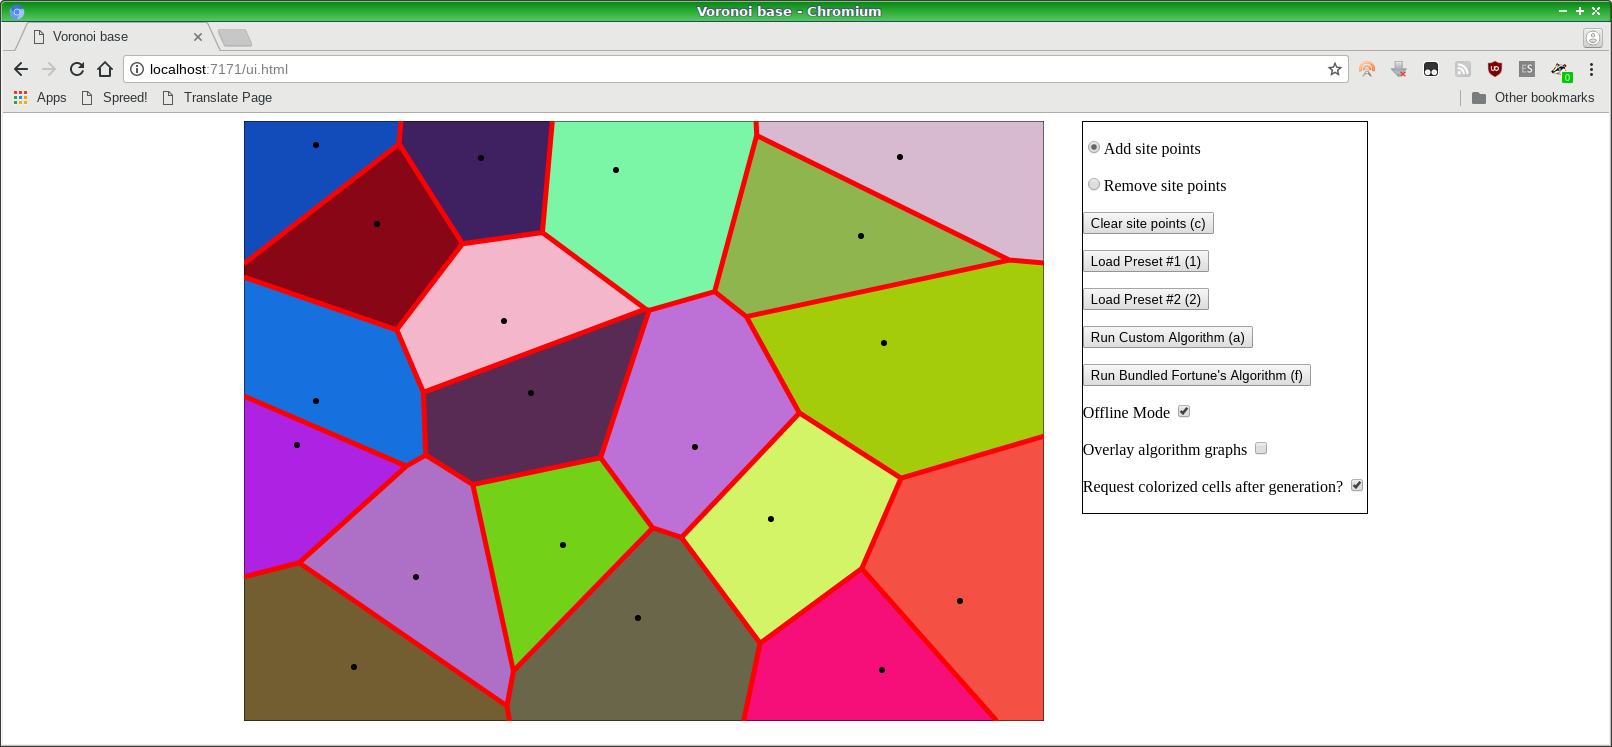
\includegraphics[width=0.99\textwidth]{screenshot.png}

\subsection*{Background Info}

The above graphic shows a complete diagram. There are several dots in the
diagram -- these represent control points, or Sites. $n$ of these are inputted
arbitrarily by a user, you are guaranteed at least 2. The Voronoi diagram is
the unique set of line segments in the rest of the graph.

Around each Site point is a set of edges, or lines, that define the Site's
Cell or polygon. The definition of the Voronoi diagram is such that for each
$(x, y)$ point within a Cell, the corresponding Site point is the closest (by
Euclidean distance) Site point. If two or more Site points are equidistant,
then that represents a boundary location for the Cells and is therefore
colored as part of a line in the diagram above.

Stated mathematically,\nl\nl
$\exists \{S_i\}$, $2 \leq i \leq n$ \nl
$\forall S_i \exists C_i$ \nl
$\forall (x,y) \in C_i$ and $\forall i \neq j$, $distBetween((x,y), S_i) < distBetween((x,y), S_j)$

\subsection*{Framework Details}

We've provided a shell in order to make your primary task as straightforward as
possible. It is delivered as a Java project that launches a local webserver on
port 7171 that you can interact with by visiting
\url{http://localhost:7171/ui.html}. The \texttt{ui.html} file is provided along with a
\texttt{ui.js} file, they provide a UI and means to interact with the server.
However, if you do not possess a Java environment, you
are free to write your code in JavaScript instead, see the next section for
details.

The Java file \texttt{CustomAlgorithm.java} is the primary file you will need to edit in
order to complete the problem statement. You are of course free to introduce new
files (and tests) as you see fit. Open source dependencies are also allowed, but
note the intent is to see what you can do directly, not just what other software you
can manipulate.

\texttt{CustomAlgorithm.java} has a method \texttt{generate()} whose role is to
populate the object's \texttt{graph} variable with new \texttt{Edge} objects. An
Edge represents a line segment, with a start point $(x_0, y_0)$ and an end point
$(x_1, y_1)$. When the client requests graph generation, it will send up the set
of Site points, and expect a set of edges in return. It will then draw the edges
for you. If, however, your Edge consists of a start and end point that is the
same, the client will draw a single pixel point for it. (Yes, this means you
could generate the diagram with just a bunch of pixel ``edges''!)

Included is a known-correct implementation of Fortune's Algorithm, an
efficient (though complicated) method of generating these. (We do not expect you
to derive and write your own version of that algorithm, fortunately there are
many ways of generating these diagrams!) It will draw the diagram in red for
you to compare your own output against. You can toggle which algorithm to use
from the client.

The client front-end defines a bounding box rectangle 800x600 pixels wide and
this information is passed up to the \texttt{boundingBox} variable in the
algorithm class. However it is resilient to drawing out of bounds. For instance,
if you returned an edge from $(-400, -300)$ to $(1600,1200)$, you will still see
a visible line as if your edge was from $(0,0)$ to $(800,600)$.

\subsection*{Framework Details (JavaScript)}

If you are not writing in JavaScript you can skip this section.\nl
The code you will need to manipulate is in \texttt{custom\_algorithm.js}.

\subsection*{Scoring Criteria}

Our intent is to keep any candidate busy for the allotted time, not to make a
single pass/fail type of problem. As such there are many ways you can make a
positive impression, even if you can't complete the problem statement as given.
You should attempt the problem statement for maximum effect, but here are some
suggestions for other things you can do instead / in addition, and you're free
to try wowing us with your own ideas here.

\newpage
\begin{enumerate}
  \item Try solving a simpler subproblem first, for example what is the diagram
    when you only have two Site points? What about only 3 points? \textbf{Make
    sure you include any partial or incremental work even if it doesn't end up in the final code
    path!}
  \item The UI is robust to out-of-bounds edges, but what if it wasn't? Would
    your code work? Can you verify that it would work? Are there other edge
    cases?
  \item We are a dev/QE hybrid team. The provided \texttt{FortuneAlgorithm.java}
    class results in a known-correct set of edges, but is it actually correct?
    How might you assess its quality?
  \item A dual graph of a voronoi diagram is a Delaunay triangularization. Can
    you generate the dual? Can you output its edges so that it draws?
  \item Can you color the graph Cells such that no two adjacent cells share the
    same color? (See \texttt{GraphColorizer.java} or
    \texttt{graph\_colorizer.js} for hints on where to start if you decide to
    try this.)
  \item If you generate the graph by plotting a bunch of points, can you take
    your set of points and construct a minimum set of edges that pass through
    all of them?
  \item How do other distance metrics besides Euclidean distance impact the
    graph?
  \item Is your code straightforward to follow?
  \item Do you understand the performance profile?
  \item If this is child's play, you can attempt your own version of Fortune's
    Algorithm, just be ready to explain it to us!

\end{enumerate}

\subsection*{Potentially Useful Formulas}

\noindent
Distance formula for the distance between two points $(x_0, y_0)$ and $(x_1,
y_1)$:
$$distance = \sqrt{(x_0 - x_1)^2 + (y_0 - y_1)^2)}$$

\noindent\nl
Midpoint formula for the midpoint between two points:
$$(x_m, y_m) = (\frac{x_0+x_1}{2}, \frac{y_0+y_1}{2})$$

\noindent\nl
Formula of a line:
$$y = mx + b$$ 
where $m$ is the line slope, $b$ is the
y-intercept, and so given $x$ you can calculate $y$.

\noindent\nl
Alternate formula of a line:
$$y = m(x-a)+b$$
where $m$ is the line slope, and the
point $(a,b)$ is any known point on the line.

\noindent\nl
Slope between two points:
$$slope = \frac{y_1 - y_0}{x_1 - x_0}$$

\noindent\nl
Perpendicular slope:
$$slope_{perp} = \frac{-1}{slope}$$

This is open book / internet, just be prepared to deeply explain everything you
do including how you arrived at writing any particularly piece of code.

\end{document}
